\chapter{Gerelateerde werken}

\begin{itemize}
	\item Bron \cite{real-time-human-pose-recognition-in-parts-from-a-single-depth-image}
	\begin{itemize}
		\item voorstel van een methode om op een accurate manier de 3D posities van de joints te bepalen, vanuit slechts één dieptebeeld, zonder temporale informatie
		\item Het bepalen van lichaamsdelen is invariant van pose, lichaamsbouw, kleren, etc...
		\item Kan runnen aan 200 fps
		\item Wordt effectief gebruikt in de Kinect software (onderzoeksteam is van Microsoft)
		\item Een dieptebeeld wordt gesegmenteerd in verschillende lichaamsdelen, aangegeven door een kleur, op basis van een kansfunctie; Elke pixel van het lichaam wordt apart behandeld en gekleurd. Een verzameling van dezelfde kleuren wordt een joint
		\item Aangezien tijdsaspect weg is, is er enkel interesse in de statische poses van een frame. Verschillen van pose in twee opeenvolgende frames is miniscuul zodat die genegeerd worden
	\end{itemize}

	\item Bron \cite{xia2012view}
	\begin{itemize}
		\item[$\vee$] Bevat bruikbare datasets van skelet-, diepte- en kleurenbeelden
		\item Ook hier praten ze over de vaak voorkomende uitdagingen: Intra-en interklasse variaties, de omgeving en de grootte van de verzameling van acties die er eigenlijk bestaan.
		\item Hier tonen ze ook weer het nut van de kinect sensor aan, en gebruiken de kinect
		\item Ze geven een nieuw algoritme om menselijke actieherkenning uit te voeren vanuit een dieptebeeld, een view-invariante representatie van poses en het systeem werkt \underline{real-time}.
		\item Histogram gebaseerde representatie van 3D poses (HOJ3D genoemd) = partitie van 3D ruimte in $n$ "bins", gebruik maken van een bolcoördinatensysteem. Selectie van 12 joints die een compacte representatie van het skelet weergeven. (hand en pols, voet en enkel worden gecombineerd).
		\item Het centrum van deze 3D ruimte is de de heup joint. Er is ook een vector $\alpha$, parallel met de grond, door de heup (van links naar rechts), en een vector $\theta$ loodrecht op de grond en door het centrum
			\begin{figure}[ht]
				\centering
			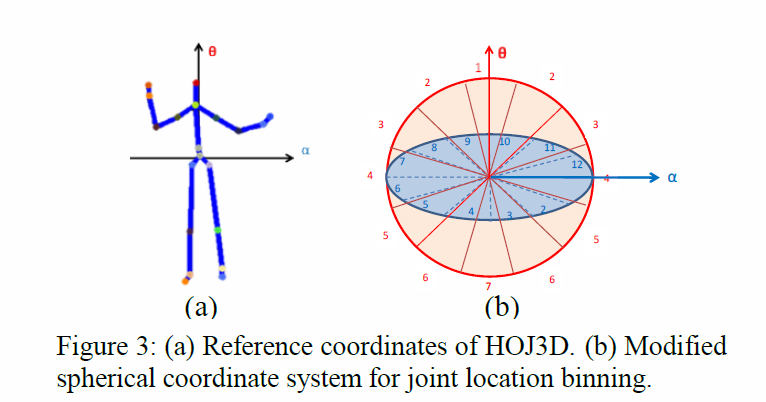
\includegraphics[width=\textwidth]{HOJ3D}
			\end{figure}
			Deze 3D ruimte (figuur 3b) wordt opgesplitst in $n$ partities.
			
			Voor $\theta$: [0, 15], [15, 45], [45, 75], [75, 105] [105, 135], [165, 180]. (7 bins)
			
			Voor $\alpha$: 30 graden voor elke bin, dus 12 bins.
			
			in totaal $7 * 12 = 84$ bins
		
			
			Via deze bolcoördinaten kan elke 3D joint gelokaliseerd worden in een unieke bin 
			\item De 3 joints die gebruikt worden om het bolcoördinatenstelsel te oriënteren staan uiteraard vast. De overige 9 joints worden onderverdeeld in één van de 84 bins. 
			
			\item Om de representatie robust te maken, wordt één enkele joint over verschillende, naburige bins verdeeld (8 buren), op basis van gewichtsfunctie:

			
			\begin{figure}[ht]
				\centering
				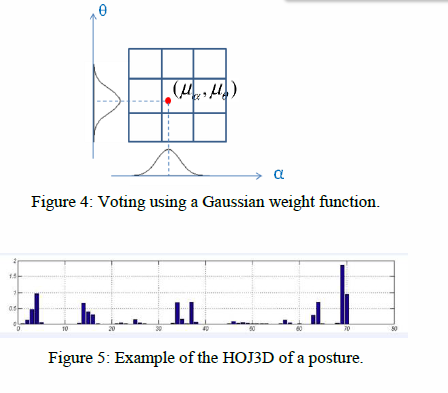
\includegraphics[width=0.5\textwidth]{HO3D_HISTOGRAM}
			\end{figure}
			
			\item Linear discriminant analysis (LDA) wordt toegepast om dominante features eruit deze histogram te halen.
			
			
			\item Ze beweren sneller te zijn dan bron \cite{action-recognition-based-bag-3d-points}
		\end{itemize}
	\item Bron \cite{action-recognition-based-bag-3d-points}
	\begin{itemize}
		\item Actieherkenning met behulp van reeksen van dieptebeelden
		\item Gaan ervan uit dat efficiënte tracking van skeletbeelden nog niet mogelijk is. (is gepubliceerd zelfde jaar dat Kinect beschikbaar was, 2010)
		\item Hun oplossing is dus niet gebaseerd op het tracken van de skeletbeelden
	\end{itemize}



	\item Bron \cite{keep-it-simple-and-sparse-real-time-action-recognition}
	\begin{itemize}
		\item s
	\end{itemize}

	\item Bron \cite{enhanced-computer-vision-with-microsoft-kinect-sensor}
	\begin{itemize}
		\item 
	\end{itemize}
\end{itemize}